\section{Background}
We provide a brief review of symbolic execution and describe the key features
of a hardware design that necessitate a new approach for symbolic execution. We
explain the recursive strategy for symbolic execution and provide some
background on the Coq proof assistant.

\subsection{Symbolic Execution}
In symbolic execution the parameters to a program's entry point are
assigned symbolic values. The program is then simulated by a symbolic execution
engine that uses the symbolic values in place of concrete literals. As
execution continues the resulting symbolic expressions propagate throughout the program's
state. A symbolic expression
\symexpression{} contains at least one symbol and may contain zero or more concrete
literals, arithmetic operators, and logical operators. Examples of
symbolic expressions include `$\alpha$' and `$\alpha + 1$,' where
$\alpha$ is a symbol used by the symbolic execution engine.

In addition to the symbolic state, the symbolic execution engine keeps track
of the \emph{path condition} (\pathcondition) for the current path of
execution. When execution begins the path condition is initialized 
to \texttrue. At each conditional branch in the program, the branching condition $b$ is evaluated. If $\pathcondition
\rightarrow b$ is valid, the $\mathtt{then}$ branch is taken and the path condition is
updated, $\pathcondition := \pathcondition \wedge b$. If $\pathcondition \rightarrow \neg b$ is valid, the $\mathtt{else}$
branch is taken and the path condition is updated, $\pathcondition := \pathcondition \wedge \neg
b$. If neither $\pathcondition \rightarrow b$ nor $\pathcondition \rightarrow \neg b$ hold, then both
branches are possible. Execution forks and each branch is explored in turn
with the path condition updated appropriately for each branch.

In general, a path condition \pathcondition{} is a conjunction of propositions involving
symbolic expressions. For example `$\pathcondition := \alpha + 1 \ge 0 \wedge \alpha < 1$' is a
possible path condition.

All the paths explored through the program form a logical tree \tree. The root represents the
program's entry point and each node of the
tree represents a line of code in the program. Associated with each node is the
(partially) symbolic state of the program and the path condition at that point
of execution. A path in the tree from root to leaf
represents a path of execution through the program.

Figure~\ref{fig:se} demonstrates the idea. 
Given the code in
Figure~\ref{fig:secode}, $\mathtt{reset}$ and $\mathtt{count}$ are initialized
with the symbolic values $r_0$ and $c_0$, respectively, and after symbolically
executing lines 1, 3, and 4 $\mathtt{count}$ may be set to the symbolic expression $c_0 +
1$ as shown in Figure~\ref{fig:setable}. The
path condition for the path through lines 1, 3, 4, 5, 6 is also shown. When execution
reaches the $\mathtt{ERROR}$ at line 6 the path condition is $\pathcondition := r_0
= 0 \wedge c_0 + 1 > 3$. This expression can then be passed to a standard,
off-the-shelf SMT solver to find a satisfying solution, say $r_0 := 0$ and $c_0
:= 3$. Substituting these values for $\mathtt{reset}$ and $\mathtt{count}$,
respectively, and executing the code from the beginning using these concrete
values would cause execution to follow the same path as was followed
symbolically. Figure~\ref{fig:setree} illustrates
the tree of paths explored in the complete symbolic execution of the
code fragment.

\begin{figure}
  \centering
  \begin{subfigure}[b]{0.3\textwidth}
    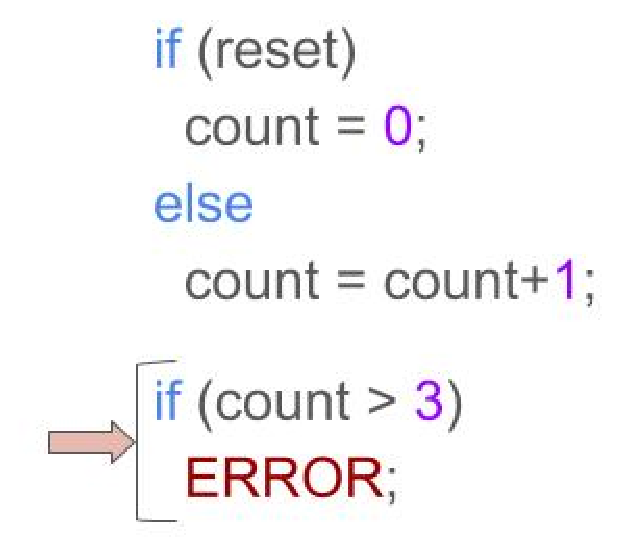
\includegraphics[trim=0 -1cm 0 0,width=\textwidth]{secode}
    \caption{Code snippet}
    \label{fig:secode}
    \end{subfigure}
  \quad
  \begin{subfigure}[b]{0.3\textwidth}
    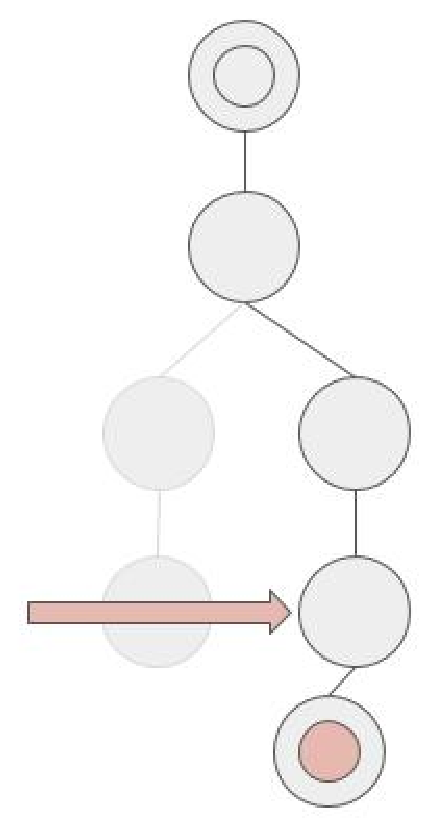
\includegraphics[trim=-2cm -.5cm 0 0,height=2in]{setree}
    \caption{Tree of program paths}
    \label{fig:setree}
    \end{subfigure}
  \quad
  \begin{subfigure}[b]{0.3\textwidth}
    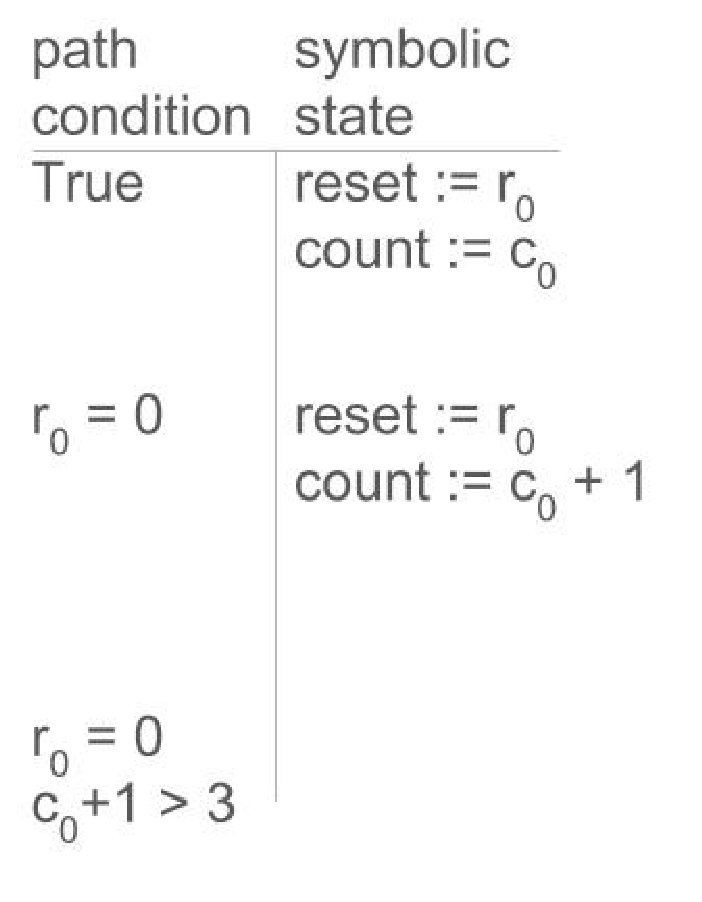
\includegraphics[height=2in]{setable}
    \caption{\pathcondition{} and symbolic state}
    \label{fig:setable}
    \end{subfigure}
  \caption{Symbolic Execution}
  \label{fig:se}
  \end{figure}

\subsection{Register Transfer Level Hardware Designs}
For their recursive strategy, Zhang et al. are targeting the symbolic execution
of a synchronous (i.e., clocked) hardware design described at the register transfer level (RTL)
of abstraction. The RTL specifies the stateful registers in the design
(implemented as flip-flops or latches) and the
combinational logic connecting those registers. A complete simulation of the design
corresponds to a single clock cycle; the symbolic execution of the design
produces a tree where the root node represents the design in a given state and
each leaf node represents a possible next-state of the design at the next clock
cycle.

The hardware design differs from software code in that it is not meant
to be executed sequentially, rather it describes a design in which updates to
different registers are all done in parallel. When run in simulation---during
which the design code must
be executed sequentially---an order of execution
is imposed and temporary variables may be introduced in order to achieve the
correct next state. The same strategy is used during symbolic execution and
therefore, while the root and leaf nodes of the resulting symbolic
execution tree correspond to valid states of the hardware design, the
intermediate nodes of the tree do not and are largely ignored. 


\subsection{Recursive Search Strategy}
The symbolic execution tree represents an exploration of the design for a single
clock cycle. But it is often desirable to find states that arise only after many
steps of execution. Because of this the complexity of the search space quickly
becomes untenable. Exploring a design for two clock cycles would require first
producing the symbolic execution tree of the design when started at the initial,
reset state, and then, for each leaf in that tree, a new symbolic execution of
the design, this time starting at the state described by the leaf node. It is to
counter this combinatorial explosion that Zhang et al. developed their recursive
search strategy. 

The gist of the recursive search strategy is to search backward from the error
state as follows. First use (forward) symbolic execution to find a state $s_i$ that has the error
state as one of its possible next-state transitions. Then use (forward) symbolic execution
to find a state $s_{i-1}$ that has $s_i$ as one of its possible next-state
transitions. This search continues until one of the found $s$'s is an initial
state of the processor. The result is a sequence of symbolic execution trees
that can be used to produce a sequence of concrete input values that take the
processor from its initial state to the error state.








%% \subsection{Recursive Search Strategy for Symbolic Execution}

%% The symbolic execution engine
%% maintains the current, partially symbolic state of the program and the current
%% \emph{path condition}. The path condition is a conjunction of propositions over
%% input and state variables that define the path through the program code taken to
%% reach the current state.


%% We model the processor as a vector $R$ of state registers $R = <r_0, r_1,
%% \ldots, r_n>$. At each step of execution (clock cycle) the valuation of each
%% register may change. New state is determined by the Boolean and bitvector
%% arithmetic combination of current state plus input values. $\forall m, r'_m =
%% \delta(R,I)$.

%% In concrete execution registers hold concrete values $(v_0, v_1, \ldots, v_n)$
%% at each clock cycle. In symbolic execution the concrete values are replaced with
%% symbolic values $(\phi_0, \phi_1, \ldots, \phi_n)$ and so are input values.
%% As execution continues, symbolic values propagate through the design.

%% The symbolic state is modeled as a tuple $\psi := (S,\pi)$ where $S$ is the
%% vector of registers containing a combination of symbolic and concrete state $S
%% := <s_0, s_1, \ldots, s_n>$. As execution continues, symbolic values propagate
%% through the design.

%% The recursive symbolic execution strategy utilizes two instantiation operations. 
%% They define them in the following way: 

%% ``Let $\mathcal{E}$ represent the symbolic exploration of one clock cycle of a processor modeled by $M$. Let $n_r = (s_r,\pi_r)$ be the root node of tree $\mathcal{E}$ and let $n_l = (s_l,\pi_l)$ be a leaf node of the same tree. 
%% Then $s_r \circ \pi_l$ represents the set of concrete states, and $s_l \circ \pi_l$ represents the set of concrete next-states, that are at the end-points of the path from $n_r$ to $n_l$.'' \cite{zhang2018recursive}

%% For our proof we let $\mathtt{concretize\_root}=  s_r \circ \pi_l$ and $\mathtt{concretize\_leaf} =  s_l \circ \pi_l$.





\subsection{Using Coq as a Verification Tool}

Coq is a formal, interactive proof assistant that allows for machine-checked proofs of systems~\cite{coqtool}. 
It implements the inductive language Gallina, which is based on the \textit{Calculus of Inductive Constructions}, a typed $\lambda$-calculus. It allows definitions of methods that can be evaluated, the expression of theorems and software specifications, and assists the user in building machine-checkable proofs. If the proof is complete, it will compile.


%There are four main structures in Coq that we use in our proof:
%\begin{itemize}
%\item \emph{Axiom} is used to express properties that do not need to be proven. These are meant to be accepted as ground truth in the system. 
%\item \emph{Definition} and \emph{Fixpoint} are used to define methods.
%\item \emph{Variable} defines local variables.
%\item \emph{Theorem} expresses a property that needs to be proven.
%\end{itemize}

 

Additionally, we make use of Coq's module system, representing different parts
of our system as modules.  There is a module defining concrete execution, a
module defining symbolic execution that includes the King properties as axioms,
and a module defining the recursive symbolic execution strategy that includes
the requirements laid out by Zhang and Sturton as axioms and the correctness property expressed as a theorem.

Our definitions and fixpoints are the methods that are implemented
in the system, such as execution of the list of trees provided by the recursive
symbolic execution tool. Our variables are system-specific variables, such as the
initial state and the error states, and they are contained in the recursive symbolic execution module as well.

We use the built-in Logic library for assistance in small proofs and the Ensembles library for assistance reasoning about finite sets. Additionally, we use the built-in List structure to represent lists of symbolic execution trees.









